\documentclass{article}
\usepackage{graphicx, tikz-cd, float, titlepic, booktabs} % Required for inserting images
\usepackage{pgfplots}
\pgfplotsset{compat=1.15}
\usepackage{mathrsfs}
\usetikzlibrary{arrows}
\usepackage{amsmath, amssymb, amsthm, amsfonts, siunitx, physics, gensymb}
\AtBeginDocument{\RenewCommandCopy\qty\SI}
\usepackage[version=4]{mhchem}
\usepackage[most,many,breakable]{tcolorbox}
\usepackage{xcolor, fancyhdr, varwidth}
\usepackage[Glenn]{fncychap}
%Options: Sonny, Lenny, Glenn, Conny, Rejne, Bjarne, Bjornstrup
\usepackage{hyperref, cleveref}
\usepackage{icomma, enumitem} %comma as decimal and continue enumerate with [resume]
\usepackage[danish]{babel}
%%%%%%%%%%%%%%%%%%%%%%%%%%%%%%
% SELF MADE COLORS
%%%%%%%%%%%%%%%%%%%%%%%%%%%%%%
\definecolor{myg}{RGB}{56, 140, 70}
\definecolor{myb}{RGB}{45, 111, 177}
\definecolor{myr}{RGB}{199, 68, 64}
\definecolor{mytheorembg}{HTML}{F2F2F9}
\definecolor{mytheoremfr}{HTML}{00007B}
\definecolor{mylenmabg}{HTML}{FFFAF8}
\definecolor{mylenmafr}{HTML}{983b0f}
\definecolor{mypropbg}{HTML}{f2fbfc}
\definecolor{mypropfr}{HTML}{191971}
\definecolor{myexamplebg}{HTML}{F2FBF8}
\definecolor{myexamplefr}{HTML}{88D6D1}
\definecolor{myexampleti}{HTML}{2A7F7F}
\definecolor{mydefinitbg}{HTML}{E5E5FF}
\definecolor{mydefinitfr}{HTML}{3F3FA3}
\definecolor{notesgreen}{RGB}{0,162,0}
\definecolor{myp}{RGB}{197, 92, 212}
\definecolor{mygr}{HTML}{2C3338}
\definecolor{myred}{RGB}{127,0,0}
\definecolor{myyellow}{RGB}{169,121,69}
\definecolor{myexercisebg}{HTML}{F2FBF8}
\definecolor{myexercisefg}{HTML}{88D6D1}
%%%%%%%%%%%%%%%%%%%%%%%%%%%%%%%%%%%%%%%%%%%%%%%%%%%%%%%%%%%%%%%%%%%%%%
% Box environments for theorems and problems
%%%%%%%%%%%%%%%%%%%%%%%%%%%%%%%%%%%%%%%%%%%%%%%%%%%%%%%%%%%%%%%%%%%%%
\setlength{\parindent}{1cm}
%================================
% Question BOX
%================================
\makeatletter
\newtcbtheorem{question}{Opgave}{enhanced,
	breakable,
	colback=white,
	colframe=myb!80!black,
	attach boxed title to top left={yshift*=-\tcboxedtitleheight},
	fonttitle=\bfseries,
	title={#2},
	boxed title size=title,
	boxed title style={%
			sharp corners,
			rounded corners=northwest,
			colback=tcbcolframe,
			boxrule=0pt,
		},
	underlay boxed title={%
			\path[fill=tcbcolframe] (title.south west)--(title.south east)
			to[out=0, in=180] ([xshift=5mm]title.east)--
			(title.center-|frame.east)
			[rounded corners=\kvtcb@arc] |-
			(frame.north) -| cycle;
		},
	#1
}{def}
\makeatother
%================================
% DEFINITION BOX
%================================

\newtcbtheorem[]{Definition}{Definition}{enhanced,
	before skip=2mm,after skip=2mm, colback=red!5,colframe=red!80!black,boxrule=0.5mm,
	attach boxed title to top left={xshift=1cm,yshift*=1mm-\tcboxedtitleheight}, varwidth boxed title*=-3cm,
	boxed title style={frame code={
					\path[fill=tcbcolback]
					([yshift=-1mm,xshift=-1mm]frame.north west)
					arc[start angle=0,end angle=180,radius=1mm]
					([yshift=-1mm,xshift=1mm]frame.north east)
					arc[start angle=180,end angle=0,radius=1mm];
					\path[left color=tcbcolback!60!black,right color=tcbcolback!60!black,
						middle color=tcbcolback!80!black]
					([xshift=-2mm]frame.north west) -- ([xshift=2mm]frame.north east)
					[rounded corners=1mm]-- ([xshift=1mm,yshift=-1mm]frame.north east)
					-- (frame.south east) -- (frame.south west)
					-- ([xshift=-1mm,yshift=-1mm]frame.north west)
					[sharp corners]-- cycle;
				},interior engine=empty,
		},
	fonttitle=\bfseries,
	title={#2},#1}{def}
\newtcbtheorem[]{definition}{Definition}{enhanced,
	before skip=2mm,after skip=2mm, colback=red!5,colframe=red!80!black,boxrule=0.5mm,
	attach boxed title to top left={xshift=1cm,yshift*=1mm-\tcboxedtitleheight}, varwidth boxed title*=-3cm,
	boxed title style={frame code={
					\path[fill=tcbcolback]
					([yshift=-1mm,xshift=-1mm]frame.north west)
					arc[start angle=0,end angle=180,radius=1mm]
					([yshift=-1mm,xshift=1mm]frame.north east)
					arc[start angle=180,end angle=0,radius=1mm];
					\path[left color=tcbcolback!60!black,right color=tcbcolback!60!black,
						middle color=tcbcolback!80!black]
					([xshift=-2mm]frame.north west) -- ([xshift=2mm]frame.north east)
					[rounded corners=1mm]-- ([xshift=1mm,yshift=-1mm]frame.north east)
					-- (frame.south east) -- (frame.south west)
					-- ([xshift=-1mm,yshift=-1mm]frame.north west)
					[sharp corners]-- cycle;
				},interior engine=empty,
		},
	fonttitle=\bfseries,
	title={#2},#1}{def}

\newtcbtheorem{theo}%
    {Theorem}{}{theorem}
\newtcolorbox{prob}[1]{colback=red!5!white,colframe=red!50!black,fonttitle=\bfseries,title={#1}}
%================================
% NOTE BOX
%================================

\usetikzlibrary{arrows,calc,shadows.blur}
\tcbuselibrary{skins}
\newtcolorbox{note}[1][]{%
	enhanced jigsaw,
	colback=gray!20!white,%
	colframe=gray!80!black,
	size=small,
	boxrule=1pt,
	title=\textbf{Note:},
	halign title=flush center,
	coltitle=black,
	breakable,
	drop shadow=black!50!white,
	attach boxed title to top left={xshift=1cm,yshift=-\tcboxedtitleheight/2,yshifttext=-\tcboxedtitleheight/2},
	minipage boxed title=1.5cm,
	boxed title style={%
			colback=white,
			size=fbox,
			boxrule=1pt,
			boxsep=2pt,
			underlay={%
					\coordinate (dotA) at ($(interior.west) + (-0.5pt,0)$);
					\coordinate (dotB) at ($(interior.east) + (0.5pt,0)$);
					\begin{scope}
						\clip (interior.north west) rectangle ([xshift=3ex]interior.east);
						\filldraw [white, blur shadow={shadow opacity=60, shadow yshift=-.75ex}, rounded corners=2pt] (interior.north west) rectangle (interior.south east);
					\end{scope}
					\begin{scope}[gray!80!black]
						\fill (dotA) circle (2pt);
						\fill (dotB) circle (2pt);
					\end{scope}
				},
		},
	#1,
}
%================================
% EXAMPLE BOX
%================================
\newtcbtheorem[number within=section]{Example}{Example}
{%
	colback = myexamplebg
	,breakable
	,colframe = myexamplefr
	,coltitle = myexampleti
	,boxrule = 1pt
	,sharp corners
	,detach title
	,before upper=\tcbtitle\par\smallskip
	,fonttitle = \bfseries
	,description font = \mdseries
	,separator sign none
	,description delimiters parenthesis
}
{ex}
%================================
% THEOREM BOX
%================================

\tcbuselibrary{theorems,skins,hooks}
\newtcbtheorem[number within=section]{Theorem}{Theorem}
{%
	enhanced,
	breakable,
	colback = mytheorembg,
	frame hidden,
	boxrule = 0sp,
	borderline west = {2pt}{0pt}{mytheoremfr},
	sharp corners,
	detach title,
	before upper = \tcbtitle\par\smallskip,
	coltitle = mytheoremfr,
	fonttitle = \bfseries\sffamily,
	description font = \mdseries,
	separator sign none,
	segmentation style={solid, mytheoremfr},
}
{th}

%%%%%%%%%%%%%%%%%%%%%%%%%%%%%%%%%%%%%%%%%%%%%%%%%%%%%%%%%%%%%%%%%
% SELF MADE COMMANDS
%%%%%%%%%%%%%%%%%%%%%%%%%%%%%%
\newcommand{\sol}{\setlength{\parindent}{0cm}\textbf{\textit{Løsning:}}\setlength{\parindent}{1cm}}
%%%%%%%%%%%%%%%%%%%%%%%%%%%%%%%%%
\usepackage[tmargin=2cm,rmargin=1in,lmargin=1in,margin=0.85in,bmargin=2cm,footskip=.2in]{geometry}\pagestyle{fancy}
\lhead{Minrui Kevin Zhou 2.b}
\rhead{Aflevering 29}

\title{Aflevering 29\\
{\Large \textbf{2.b mat A}}}
\author{Kevin Zhou}
\date{\today}

\begin{document}
\maketitle
\section*{Bedømmelseskriterier:}
\begin{itemize}
    \setlength\itemsep{3cm}
    \Large
    \item  Redegørelse og dokumentation for metode
    \item Figurer, grafer og andre illustrationer
    \item Notation og layout
    \item Formidling og forklaring
\end{itemize}
\pagebreak
\begin{question}{}{}
 En vektorfunktion $\va{r}: \mathbb{R} \to \mathbb{R}^2$ er givet ved
  \[
  \va{r}(t)=\mqty(2t^3-t^2\\ 2t^2-2t) 
  \] 
  \begin{itemize}
    \item[a.] Bestem en parameterfremstilling for tangenten til parameterkurven for $\va{r} $ i punktet $P(0,4)$.
  \end{itemize}
\end{question}
\sol \\
\textbf{a.}
Vi løser først ligningen $x(t)=0$ mht. $t$ for at finde $t$-værdien, når $\va{r}(t)=P$. 
\begin{equation*}
\begin{split}
  x(t)=0 &\iff 2t^3-t^2=0 \\ 
  &\iff t^2 \cdot \left(2t-1\right) =0\\ 
  &\iff t=0 \lor t=\frac{1}{2}
\end{split}
\end{equation*}
Vi indsætter disse værdier i $y(t)$.
\begin{equation*}
\begin{split}
  t=0 &\implies y(t)=2 \cdot 0 - 2 \cdot 0=0\\ 
  t=\frac{1}{2} &\implies y(t)=\frac{2}{4}-1=-\frac{1}{2} 
\end{split}
\end{equation*}
Ved indsættelse af disse værdier i $y(t)$ ses det, at ingen af $y$-værdierne er 4.
Altså må det gælde, at $P\notin Vm(\va{r})$.
\begin{question}{}{}
  En vektorfunktion $\va{s}:\mathbb{R}\to \mathbb{R}^2$ er givet ved 
  \[
  \va{s}(t)=\mqty(t^3-2t\\ t^2)
  \] 
  Punktet $P(4,4)$ ligger på parameterkurven for $\va{s}$. 
  \begin{itemize}
    \item[a.] Bestem parameterværdien $t$ hørende til $P$. 
    \item[b.] Gør rede for, at linjen $l:2x-5y+12=0$ er en tangent til parameterkurven for $\va{s}$ i punktet $P$. 
  \end{itemize}
\end{question}
\sol \\
\textbf{a.}
Vi løser da først ligningen $y(t)=4$.
\begin{equation*}
\begin{split}
  t^2=4 \iff t=2 \lor t=-2
\end{split}
\end{equation*}
Vi regner $x(t)$ med disse $t$-værdier.
\begin{equation*}
\begin{split}
  x(2)&=2^3-2 \cdot 2=4\\ 
  x(-2)&=(-2)^3+2 \cdot 2=-4 \neq 4
\end{split}
\end{equation*}
Altså har vi $\va{s}(2)=(4,4)$. 
Parameterværdien hørende til $P$ må da være $2$. \\[1ex]
\textbf{b.}
Vi finder først den afledede funktion for $\va{s} $.
\begin{equation*}
\begin{split}
  \va{s}'(t)=\mqty(3t^2-2\\ 2) 
\end{split}
\end{equation*}
Vi finder retningsvektoren for tangenten i punktet $P$, der blot er værdien af funktionen $\va{s}'$ når $t=2$. 
\begin{equation*}
\begin{split}
  \va{s}'(2)&=\mqty(3 \cdot 2^2-2\\ 2) \\ 
  &=\mqty(10\\ 2) 
\end{split}
\end{equation*}
Imidlertid aflæser vi fra linjens ligning, at $\va{n} =\mqty(2\\ -5) $ er en normalvektor til $l$. 
Siden der gælder, at
\begin{equation*}
\begin{split}
  \va{n} \cdot \va{s}'(2)&=10 \cdot 2-2 \cdot 5\\ 
  &=0
\end{split}
\end{equation*}
så må $l$ være parallel med tangenten til parameterkurven i punktet $P$ (for retningsvektoren er ortogonal med normalvektoren). 
Vi mangler nu blot at vise, at $P \in l$.

Da ser vi, at
\[
2 \cdot 4-5 \cdot 4 + 12=0
\] 
og $P$ må være et element i $l$. 
Altså har vi nu vist, at $l:2x-5y+12=0$ er en tangent til parameterkurven for $\va{s} $ i punktet $P$. 
\begin{question}{}{}
  En vektorfunktion $\va{s}:[-2,5;2,5]\to \mathbb{R}^2$ er givet ved 
  \[
  \va{s}(t)=\mqty(t^3-3t\\ -t^4+4t^2) 
  \] 
  Parameterkurven for $\va{s} $ har tre dobbeltpunkter. 
  Det oplyses, at et af dobbeltpunkterne har $t$-værdien 
  \[
  t=\frac{1}{2}\left(\sqrt{6} +\sqrt{2} \right) 
  \] 
  \begin{itemize}
    \item[a.] Bestem koordinatsættet til dette dobbeltpunkt.
  \end{itemize}
  Det oplyses, at der er et dobbeltpunkt i $P(-\sqrt{2},1)$.
  \begin{itemize}
    \item[b.] Bestem $t$-værdierne hørende til dette dobbeltpunkt.
  \end{itemize}
  Det oplyses, at det sidste dobbeltpunkt ligger på andenaksen.
  \begin{itemize}
    \item[c.] Bestem $t$-værdierne hørende til dette dobbeltpunkt.
  \end{itemize}
\end{question}
\sol \\
\textbf{a.}
Vi finder koordinatsættet til dette punkt ved at regne $\va{s}(t)$.
\begin{equation*}
\begin{split}
  \va{s}\left(\frac{1}{2}\left(\sqrt{6} +\sqrt{2} \right)\right)&=\mqty(\frac{1}{8}\left(\sqrt{2} +\sqrt{6} \right)^3-\frac{3}{2}\left(\sqrt{2} +\sqrt{6} \right)\\ 1) 
\end{split}
\end{equation*}
Altså er koordinatsættet til dette dobbeltpunkt $\left(\frac{1}{8}\left(\sqrt{2} +\sqrt{6} \right)^3-\frac{3}{2}\left(\sqrt{2} +\sqrt{6} \right),\;1\right) $. \\[1ex]
\textbf{b.}
Med hensyn til dette dobbeltpunkt har vi da følgende ligning, der løses med CAS (se \cref{fig:CAS}).
\begin{equation*}
\begin{split}
  t^3-3t=-\sqrt{2} \land -t^4+4t^2=1 \implies  t = \frac{-\sqrt{2} + \sqrt{6}}{2}\lor t = \frac{-\sqrt{2} - \sqrt{6}}{2}  
\end{split}
\end{equation*}
Altså er $t$-værdierne hørende til dette dobbeltpunkt $\frac{-\sqrt{2} + \sqrt{6}}{2}$ og $ \frac{-\sqrt{2} - \sqrt{6}}{2}$. \\[1ex]
\textbf{c.}
Siden dobbeltpunktet ligger på andenaksen, så må $x(t)=0$.
Vi løser denne ligning med hensyn til $t$.
\begin{equation*}
\begin{split}
  t^3-3t=0 &\iff t(t^2-3)=0\\ 
  &\iff t=0 \lor t=\sqrt{3} \lor t=-\sqrt{3} 
\end{split}
\end{equation*}
For vektorfunktionen har vi at $y(t)=-t^4+4t^2$.
Det er da nemt at se, at 
\[
y(\sqrt{3} )=y(-\sqrt{3} )\neq y(0)
\] 
Altså må $t$-værdierne hørende til dobbeltpunktet på andenaksen være $\sqrt{3} $ og $-\sqrt{3} $.
\begin{figure}[H]
\begin{center}
  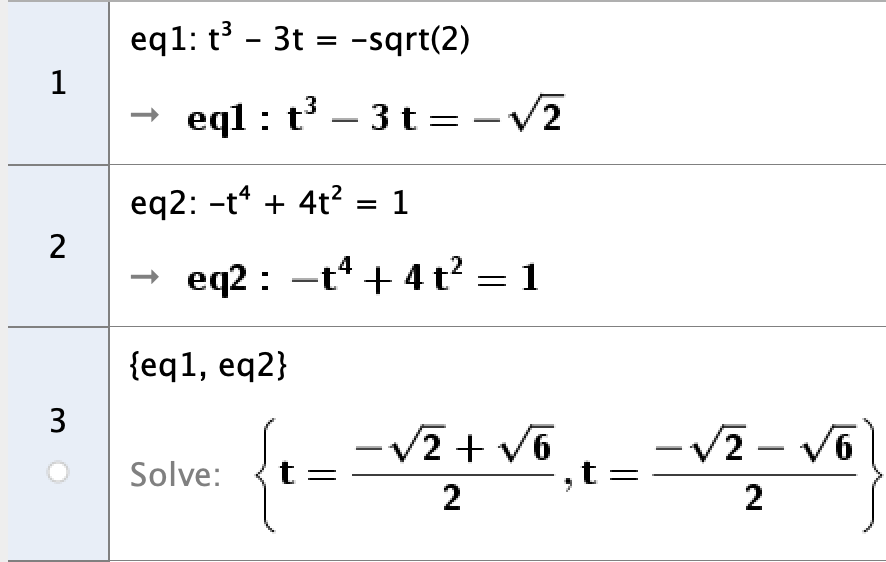
\includegraphics[width=\textwidth]{CAS.png}
\end{center}
\caption{Ligningssystemet løses med CAS}
\label{fig:CAS}
\end{figure}
\end{document}
